\documentclass{article}
\usepackage[utf8]{inputenc}
\usepackage[T1]{fontenc}
\usepackage{CJKutf8}

\usepackage{multirow}
\usepackage{multicol}
\usepackage{listings}

\usepackage{geometry}
\geometry{b5paper}
\usepackage{graphicx}

\title{CS572 Project \#1b Report}
\author{Heyan Huang}

\usepackage{geometry}
%\geometry{left=0cm,right=0cm,top=0.1cm,bottom=0cm}

\newenvironment{narrow}[2]{% 
\begin{list}{}{% 
\setlength{\topsep}{0pt}% 
\setlength{\leftmargin}{#1}% 
\setlength{\rightmargin}{#2}% 
%\setlength{\listparindent}{\parindent}% 
%\setlength{\itemindent}{\parindent}% 
\setlength{\parsep}{\parskip}% 
}% 
\item[]}{\end{list}} 
%\begin{narrow}{0.35in}{0in}  \end{narrow}
\begin{document}
\begin{CJK}{UTF8}{gbsn}
\maketitle


\lstset{language=c++,
numbers=left, 
numberstyle=\tiny, 
tabsize=4,
%keywordstyle=\color{blue!70}, commentstyle=\color{red!55!green!55!blue!55}, 
%frame=shadowbox, 
%rulesepcolor=\color{red!20!green!20!blue!20},
escapeinside=``, 
%xleftmargin=0em,xrightmargin=0em, aboveskip=0.5em
extendedchars=false %这一条命令可以解决代码跨页时,章节标题,页眉等汉字不显示的问题
}


\section{Algorithm Descriptions}

\subsection{Data Structure}
\begin{itemize}
  \itemsep=-3pt
\item In this project, I have implemented Object-Oriented(OO) design as suggested by Dr. Soule. 

\item There are two classes. 
  \begin{itemize}
    \itemsep=-3pt

  \item The base class is called Individual, indcludes member data indicating Individual point with a 30-dimension(length) dynamically allocated float values array, and a float fitness value.
  \item The publicly derived class is called Population, indcludes member data indicating a int variable size storing the Population size, and a pointer to Individual dynamic array of Population size, pointer to dynamic int array for storing sample index, and pointer to float array storing the weight matrix for Roulette wheel selection method, together with constructor, copy constructor, destructor functions and some member functions.
  \end{itemize}

\item The base class pointer is not necessary. As the first time of implementing some OO design, I tried to manage pointer, but it ended up to be an fair experience. The advantages and disadvantages will be discussed in the discussion section. 
\end{itemize}


\subsection{Algorithm Step-Wise Descriptions}

\subsubsection{Generate Base Individual Class}
To make the implementation step-wise, I Generated the base class and make sure it works first.
\begin{itemize}
  \itemsep=-3pt

\item Data members include float variable fitness, and a pointer to float array of dynamic size;
\begin{lstlisting}[language=c++]
    float* point;      // pointer to dynamic array of dimension p
    float fitness;     // store fitness value for the point
\end{lstlisting}

\item Since I have pointer included in my interface, I need to develop my own constructor, destructor, copy constructor, and assignment operator, as well as declaring the destructor and assignment operator virtual for later on potential dynamic binding at run time. 
\begin{lstlisting}[language=c++]
Individual::Individual(): fitness(INF) {
    point = new float[p];
}

Individual::Individual(const Individual &orig): fitness(orig.fitness)
{ }

Individual& Individual::operator=(const Individual &rhs) {
    // I didn't really use this function, it's complicated
    Individual* pOrig = this;
    point = new (Individual(*rhs)).point;
    delete [ ] pOrig;

    Individual temp(rhs);

    // need define my own specialized std::swap template,
    // template<class T> std::swap(T& a, T& b) {  }
      
    // instant the template with Individual object before use
    // template< > std::swap<Individual>(
    //	              Individual a, Individual b)
    // {a.swap(b); ...}
    std::swap(temp);
      
    return *this;
}

Individual::~Individual() {
    delete [ ] point;
}
\end{lstlisting}

\item Initialized Individual point by Generate random float value for each dimension within valid range; And since point got Initialized already, calculate the fitness and store it.
\begin{lstlisting}[language=c++]
    void Individual::generate() {
      for (int i = 0; i < p; ++i) {
        if ( (rand()%100/100.0) >= 0.50 )
        point[i] = rand() % 7 - (rand() % 100000)/100000.0;
        else
        point[i] = -rand() % 7 + (rand() % 100000)/100000.0;
        while (point[i] < sphl || point[i] > sphh) {
          if ( (rand()%100/100.0) >= 0.50 )
          point[i] = rand() % 7 - (rand() % 100000)/100000.0;
          else
          point[i] = -rand() % 7 + (rand() % 100000)/100000.0;
        } 
      }     
      fitness = getFitness();
    }
\end{lstlisting}

\item Write helper function print() to help visualization the Results.
  \begin{lstlisting}[language=c++]
    void Individual::print() {
      for (int i = 0; i < p; ++i) {
        printf("%5.5f ", point[i]);
        if (i % 5 == 4)
        printf(" ");
        if (i % 10 == 9)
        printf("\n");
      }
      printf("\n");
    }
  \end{lstlisting}

\item Mutate Individual as will have overloaded function for subclass.
  \begin{lstlisting}[language=c++]
    void Individual::mutate() {
      float delta, temp;

      for (int i = 0; i < p; ++i) {
        delta = ( rand() % 100000 ) / 100000.00000;
        if ( (rand()%100/100.0) < 0.5)  // pos
        temp = point[i] + delta;
        else                            // neg
        temp = point[i] - delta;
        while (temp < sphl || temp > sphh) {
          delta = ( rand() % 100000 ) / 100000.00000;
          if ( (rand()%100/100.0) < 0.5) // pos
          temp = point[i] + delta;
          else                          // neg
          temp = point[i] - delta;
        } // while
        point[i] = temp;
      }
      
      fitness = getFitness();
    }
  \end{lstlisting}
\end{itemize}
base class Individual interface is listed as below: 
\lstinputlisting[language=c++]{individual.h}

\subsubsection{Generate Derived Population Class}
\begin{itemize}
  \itemsep=-3pt

\item Data members include int variable for Population size, pointer to Individual dynamic array, as well as a pointer to dynamical int array for Tournament selection method store the sample indexes. 
  \begin{lstlisting}[language=c++]
    int size;
    Individual* popu;
    int* idxArray;
  \end{lstlisting}

\item Data member includes pointer, so self-develop constructor, destructor, copy constructor and assignment operator, I guess I may need overload "->" and "[ ]" operators as well. But since pointers got crazy already, I tried to avoid complexity. 
  \begin{lstlisting}[language=c++]
    Population::Population(int n): size(n) {
      popu = new Individual[size];
    }

    Population::Population(const Population &orig):
    Individual(orig), size(orig.size) { }

    Population& Population::operator=(const Population &rhs) {
      if (this != &rhs) {
        Individual::operator=(rhs);   // assigns the base part
        size = rhs.size;
      }
      return *this;
    }

    Population::~Population() {
      // FOR loop delete individuals separately to make safe
      for (int i = 0; i < size; ++i) 
      popu[i].Individual::~Individual();	 
      delete [] idxArray;
    }
  \end{lstlisting}

\item Generate the population by generate Individuals Population size times
  \begin{lstlisting}[language=c++]
    void Population::generate() { // generate population
      for (int i = 0; i < size; ++i) {
        popu[i].Individual::generate();
      }
    }
  \end{lstlisting}

\item Wrote both selection methods for Tournament and Roulette Wheel to get better understanding. 
  \begin{itemize}
    \itemsep=-3pt
  \item Tournament Selection
    \begin{lstlisting}[language=c++]
      void Population::genRanIndi(int n) {
        idxArray = new int[n];
        for (int i = 0; i < n; ++i) 
        idxArray[i] = rand() % size;
      }

      int Population::tourSelection(int len) {
        int winIdx = rand() % len;
        float winFitness = popu[idxArray[winIdx]].fitness;
        int temp;
        float tempFitness;
        for (int i = 0; i < len; ++i) {
          temp = idxArray[i];
          tempFitness = popu[temp].fitness;
          if (tempFitness < winFitness) {
            winFitness = tempFitness;
            winIdx = temp;
          }
        }
        return winIdx;
      }
    \end{lstlisting}

  \item Roulette Wheel Selection
    \begin{lstlisting}[language=c++]
      int Population::roulSelection() {
        float* weight = new float[size];

        float minFitness = Population::minFitness();
        float tempFitness;
        float sumFitness;
        bool negFlag = false;
        float sum = 0.0;

        if ( minFitness < 0.000001)
        negFlag = true;

        if (negFlag) {
          sumFitness = (avgFitness() - minFitness)*size;
          for (int i = 0; i < size; ++i) {
            tempFitness = popu[i].fitness - minFitness;
            sum += -minFitness + tempFitness;
            weight[i] = (float) (sum / sumFitness );
          }
        } else {
          sumFitness = avgFitness()*size;
          for (int i = 0; i < size; ++i) {
            tempFitness = popu[i].fitness;
            sum += tempFitness;
            weight[i] = (float) (sum / sumFitness );
          }
        }

        float prob = ( rand() % 1000 ) / 1000.0;
        for (int i = 0; i < size; ++i) {
          if (weight[i] < prob && weight[i+1] >= prob) {
            delete [] weight;
            return i+1;
          }
        }

        delete [] weight;
        return -1;
      }
    \end{lstlisting}
  \end{itemize}

\item helper functions include generate random Individuals, get Min and Max fitness functions, printer functions as well as mutateAll to mutate the whole population.
  \begin{lstlisting}[language=c++]
    void Population::mutateAll() { 
      for (int i = 0; i < size; ++i) {
        popu[i].Individual::mutate();
      }
    }

    float Population::minFitness() {
      float minFitness = popu[0].fitness;
      float tempFitness;
      for (int i = 1; i < size; ++i) {
        tempFitness = popu[i].fitness;
        if (tempFitness < minFitness)
        minFitness = tempFitness;
      }
      return minFitness;
    }

    int Population::maxFitness() {
      float maxFitness = popu[0].fitness;
      float tempFitness;
      int worIdx = 0;
      for (int i = 1; i < size; ++i) {
        tempFitness = popu[i].fitness;
        if (tempFitness - maxFitness > 0.00001) {
          maxFitness = tempFitness;
          worIdx = i;
        }
      }
      return worIdx;
    }

    float Population::avgFitness() {
      float avgFitness = 0.0;
      for (int i = 0; i < size; ++i) {
        avgFitness += popu[i].fitness;
      }
      avgFitness = (float) (avgFitness / size);
      return avgFitness;
    }

    void Population::printRanIndi(int len) {
      for (int i = 0; i < len; ++i)
      printf("%d ", idxArray[i]);
      printf("\n");
    }
  \end{lstlisting}
\end{itemize}

Derived class Population interface is listed as followed: 
\lstinputlisting[language=c++]{population.h}

\subsubsection{Ensemble Genetic Algorithm}
In this Project, since I am trying to implement an OO design together with handling pointer, to try to avoid complexity, I have choose to use the easier to implemented Steady-state Algorithm at the cost and risk of slowing down and may not get the expected Results within limited time frame.

\begin{itemize}
  \itemsep=-3pt
\item Instance a Population object of Population size 100;
  \begin{lstlisting}[language=c++]
    int popuSize = 100;

    Population* popu = new Population(popuSize);
    popu->generate();
  \end{lstlisting}

\item Using Tournament selection method selected sample size of 5 Individuals during each generation; 
  \begin{lstlisting}[language=c++]
    int sampleSize = 5;
    int* idxArray = new int[sampleSize];
    int winIdx;

    popu->genRanIndi(sampleSize);
    idxArray = popu->idxArray;
    // popu->printRanIndi(sampleSize);
    
    winIdx = popu->tourSelection(sampleSize);
  \end{lstlisting}

\item Compare sample fitnesses and keep the elite Individual untouched into new generation. Trying to speed up the evolution, I replaced the worst Individual in each parent generation with the mutated version of previously found sample elite Individual. 
  \begin{lstlisting}[language=c++]
    void Population::newGen(int winIdx) {
      // keep sample elite
      // replace worst population individual with mutated elite

      int worIdx = maxFitness();
      for (int i =0; i < p; ++i) {
	popu[worIdx].point[i] = popu[winIdx].point[i];
	popu[worIdx].fitness = popu[winIdx].fitness;
      }
      popu[winIdx].Individual::mutate();
    }

    popu->newGen(winIdx);
  \end{lstlisting}

\item I loop through these steps trying to approach the final steady state. Loop will eventually end when best Individual get the fitness less than 0.0001.
  \begin{lstlisting}[language=c++]
    bool Population::reachBest() {
      float minF = minFitness();
      if (minF < 0.0001) {
	for (int i = 0; i < size; ++i) {
          if (popu[i].fitness == minF)
          printf("Best individual: \n");
          popu[i].Individual::print();
	}
	return true;
      }
      return false;
    }

    int counter = 0;
    while(!popu->reachBest()) {
      popu->genRanIndi(sampleSize);
      idxArray = popu->idxArray;
      popu->printRanIndi(sampleSize);
      
      winIdx = popu->tourSelection(sampleSize);

      popu->newGen(winIdx);
      ++counter;
    }
  \end{lstlisting}
\end{itemize}

The pseudo-algorithm is listed followed:  % modify here
\begin{lstlisting}[language=c++]

Generate a population of size 100

Loop until best Individual reaches threshold fitness value
    record the best Individual index, point, fitness
    loop do

        // pick elite Individual from random sample
        randomly select a sample of 5, save Population indexes as value
        winner Fitness = Sample[0].fitness
        winner index = sample[0]
        Loop ( sample size - 1 ) times
            temp Fitness =  Sample[i].fitness;
            if temp Fitness better than winner Fitness
                winner Fitness = temp Fitness
                winner index = temp index
        return win index

        // Get worst Individual index from Population:  
        worst Fitness = Population[0].fitness
        worst index = 0
        Loop population size -1 times
            temp Fitness = Population[i].fitness;
            if temp Fitness worst than worst Fitness
                worst fitness = temp Fitness
                worst index = temp index
        return worst index

        // generate new child Population
        maintain current Population unchanged yet
        replace worst Population Individual with elite Individual
        mutate elite sample Individual in place, update its fitness 

    End loop
\end{lstlisting}


\subsection{Detail Attention: }
\begin{itemize}
  \itemsep=-3pt
\item Check the range of the mutated dimensions. Each mutated dimension must be within the range of function definition. 
\item In class constructors, since I have to deal with pointers, constructor does only allocate memory space job. And corresponding, in the destructor, I will have to manually release system resource to delete [] the pointer to float array for Individual::point, Population::weight, Population::popu, Population::idxArray for Tournament selection sample indexes. 
\item I had thought by mutating all the other parent Individuals (elite kept untouched, worst got replaced by mutated elite, all the others mutated slightly as well (just like we have mutated the elite Individual) trying to speed up the evolution, but it turned out that most possible the mutation to other Individuals will pull the evolutionary trend to the opposite direction. 
\item When replace worst Individual with mutated version of elite Individual, since they are pointed by pointer, I will have to conduct deep copy to ensure parent Population and child Population is on the same memory address, which also produces the trouble of frequent memory swap (and potentially increases cache miss rates?).  
\item By OO design, I have included the fitness float variable to record the fitness. So in my Steady-state Algorithm implement, when I deep copy my elite Individual to the worst Individual memory place, I need to deep copy the pointer to 30-dimension point, and I would also need to copy the elite's fitness as well. similarly, when I mutate my elite a little bit within each generation, I would also need to recalculate and update the fitness value accordingly for the mutation happened. 
\end{itemize}


\section{Results}
Compared with the Generational Algorithm, Steady-state Algorithm is very slow because during each generation change, only the worst Population Individual got mutated.

My randomly generated Population best fitness is initialized and calculated to be around 200, after some generations, the best fitness dropped down pretty fast. But the program has run hours and hours in order to reduce the best fitness down from above 3 to below it. 

I have copied and pasted the terminal last page as an indication that the Algorithm works. 
\begin{multicols}{2}
\begin{itemize}
\itemsep=-3pt
\item 69 61 62 2 72 
\item winFitness: : 2.67058
\item worIdx 1st: 43
\item 
\item 56 86 54 18 54 
\item worIdx 1st: 61
\item 
\item 13 14 40 57 81 
\item winFitness: : 3.41477
\item winFitness: : 3.20928
\item worIdx 1st: 4
\item 
\item 67 15 29 65 8 
\item winFitness: : 3.10817
\item winFitness: : 3.03638
\item worIdx 1st: 40
\item 
\item 94 6 53 14 97 
\item winFitness: : 3.32845
\item winFitness: : 2.96758
\item worIdx 1st: 29
\item 
\item 28 14 87 30 72 
\item winFitness: : 3.41477
\item winFitness: : 2.93997
\item worIdx 1st: 53
\item 
\item 26 92 62 94 45 
\item winFitness: : 2.66032
\item worIdx 1st: 87
\item 
\item 16 19 22 88 5 
\item worIdx 1st: 26
\item 
\item 48 48 19 36 49 
\item winFitness: : 3.40592
\item winFitness: : 3.26048
\item winFitness: : 3.23172
\item worIdx 1st: 0
\item 
\item 52 63 17 30 15 
\item winFitness: : 3.35991
\item winFitness: : 3.17226
\item worIdx 1st: 49
\item 
\item 93 68 88 57 74 
\item winFitness: : 3.19646
\item worIdx 1st: 30
\item 
\item 10 5 62 63 84 
\item winFitness: : 3.20610
\item winFitness: : 3.03444
\item worIdx 1st: 93
\item 
\item 37 88 30 11 27 
\item winFitness: : 3.17233
\item worIdx 1st: 62
\item 
\item 64 87 68 39 15 
\item winFitness: : 2.66032
\item worIdx 1st: 37
\item 
\item 82 95 27 37 80 
\item winFitness: : 3.28034
\item winFitness: : 2.66032
\item worIdx 1st: 87
\item 
\item 84 78 62 90 2 
\item worIdx 1st: 37
\item 
\item 39 73 87 4 66 
\item winFitness: : 2.66032
\item worIdx 1st: 4
\item 
\item 54 61 95 26 54 
\item worIdx 1st: 87
\item 
\item 44 48 2 96 96 
\end{itemize}
\end{multicols}

Since the program had run hours to reach the minimum fitness of 3.0 for the best individual, I don't want to repeat the work in order to trace it. 

Ideally, if I just generate the initial 1000 generations, and trace the best Sample Individual fitness, together with specific generation's average fitness, by plotting them, I would get a good idea about the Algorithm to see if it works. 
\begin{lstlisting}[language=c++]
  while (counter < 1000) {
    popu->genRanIndi(sampleSize);
    idxArray = popu->idxArray;
    //popu->printRanIndi(sampleSize);
    
    winIdx = popu->tourSelection(sampleSize);

    popu->newGen(winIdx);
    ++counter;

    if (counter % 10 == 0)
    printf("%d\t%4.5f\t%4.5f\n",counter,popu->minFitness(),popu->avgFitness());
  }
\end{lstlisting}

%\includegraphics[width=\textwidth]{min}
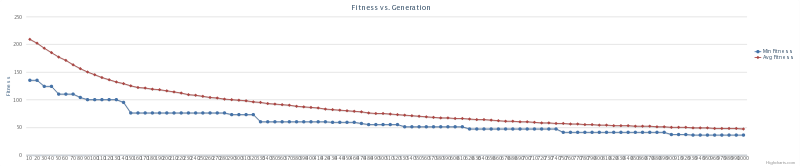
\includegraphics[width=\textwidth]{chart}

Form the scatter plot of first 1000 generations, get sample from every 10 generation, we can see the trend that the Algorithm is working perfectly. minimum fitness curve and Population average fitness curve are extending towards the same trend, and they are not separated too far away as well. And we can also see the fact that the Algorithm evolves slowly. 

\section{Conclusions}
\begin{itemize}
\itemsep=-3pt
\item Genetic Algorithm is good evolutionary Algorithm to solve some problem that is difficult for regularly-based methods.
\item Specifically, Steady-state Algorithm is slow compared with generational Algorithm. 
\end{itemize}

\section{Discussion}
As the first trial of implementation of an OO design, just like the Decision tree project I have done for Artificial Intelligence course last spring semester, I consider this one is barely an experience. I tried to use pointer and dynamic allocation, but later on, when things got complicated, I had to give up and figure out work around solutions in order to finish the project. The currently working version is simply mutate one Individual each generation, but when we require more mutations, and more generations, or more generally speaking, when I will have multiple inheritance, this design will still produce problems. And even for this current design, I still don't think it is a good design at all. 

Possible solutions to enhance the design and implementation from easy to difficult ones are listed in order in my point of view. 
\begin{itemize}
\itemsep=-3pt
\item Since the dynamic allocation is not necessary any way, simply allocate fixed size of arrays. Difficulties and issues will all go away. 
\item I can still keep my base class dynamic allocation, but for subclass, instead of using dynamic allocation again, choose standard containers like vector to store Individuals as the Population. vector will handle the memory related issues by its own destructor or member functions. 
\end{itemize}


\end{CJK}
\end{document}